\section{Federn}
\subsection{Grundlagen}

\hrule
% Hook'sches Gesetz
\begin{eeqn}{Hook'sches Gesetz}
	\begin{align}
		&\text{Normalfedern:}  &\quad  F &= c\cdot x & [c] &=\text{N/mm}\\
		&\text{Torsionsfedern:}&\quad  M &= c\cdot \alpha & [c] &=\text{Nmm}
	\end{align}
\end{eeqn}

% Federarbeit
\begin{eeqn}{Federarbeit}
	\begin{align}
		&\text{Normalfedern:}  &\quad W = \frac{1}{2} \cdot c \cdot x^2 \\
		&\text{Torsionsfedern:}&\quad  W = \frac{1}{2} \cdot c \cdot \alpha^2
	\end{align}
\end{eeqn}

% Zusammengeschaltete Federn: Reihenschaltung
\begin{eeqn}{Reihenschaltung}
	\begin{align}
		\frac{1}{c_\text{ges}} = \frac{1}{c_1} + \frac{1}{c_2} + \dots + \frac{1}{c_\text{n}}
	\end{align}
	Für die Reihenanordnung von Federn gilt die Bedingung, dass auf alle beteiligten Federn die selbe Kraft wirkt. ($F_1 = F_2 = \dots = F_\text{n}$)
\end{eeqn}

% Zusammengeschaltete Federn: Parallelschaltung
\begin{eeqn}{Parallelschaltung}
	\begin{align}
		c_\text{ges} = c_1 + c_2 + \dots + c_\text{n}
	\end{align}
	Für die Reihenanordnung von Federn gilt die Bedingung, dass alle beteiligten Federn den selben Weg zurücklegen. ($s_1 = s_2 = \dots = s_\text{n}$)
\end{eeqn}

\begin{figure}[H]
	\centering
	\begin{minipage}[b]{0.30\linewidth}
		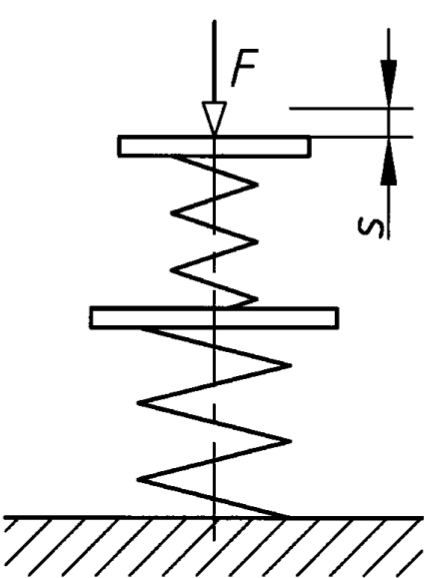
\includegraphics[width=\linewidth]{federn/reihenschaltung}
		\vspace{3.6mm}
		\caption*{Reihenschaltung}
	\end{minipage}
	\begin{minipage}[b]{0.43\linewidth}
		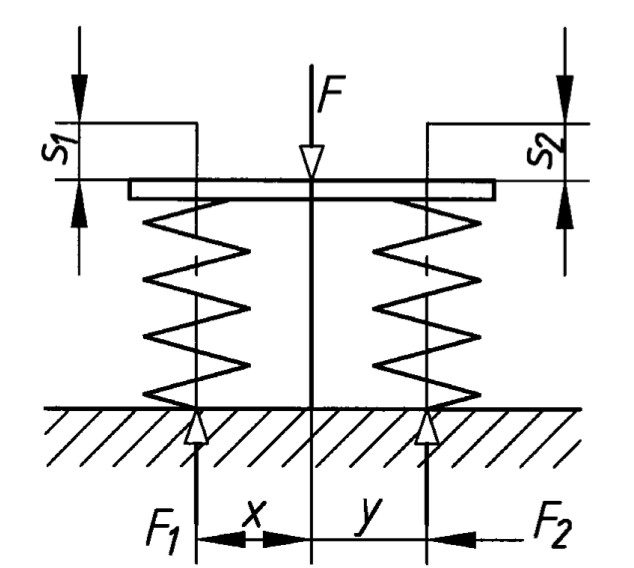
\includegraphics[width=\linewidth]{federn/parallelschaltung}
		\caption*{Parallelschaltung}
	\end{minipage}
\end{figure}


\pagebreak

\subsection{Blattfedern}
\begin{vardef}
	\item[$b$] maximale Breite der Feder.
	\item[$b'$] minimale Breite der Feder.
	\item[$b_0$] Breite der geschichteten Blattfeder.
	\item[$z$] Gesamtzahl der Blätter.
	\item[$z'$] Anzahl der Blätter mit der Gesamtlänge $L$.
	\item[$s$] Dicke der Feder.
	\item[$q_1$] Korrekturfaktor zur Berücksichtigung der Bauform
	\item[$f$] Federweg
\end{vardef}

\begin{tabularx}{\textwidth}{m{15mm}m{17mm}m{20mm}m{20mm}XX}
    \toprule
		Typ & $b(x)$ & $W_\text{ax}(x)$ & $\sigma_\text{B}(x)$ & $\sigma_\text{B,max}$ & $q_1$ \\ \midrule
		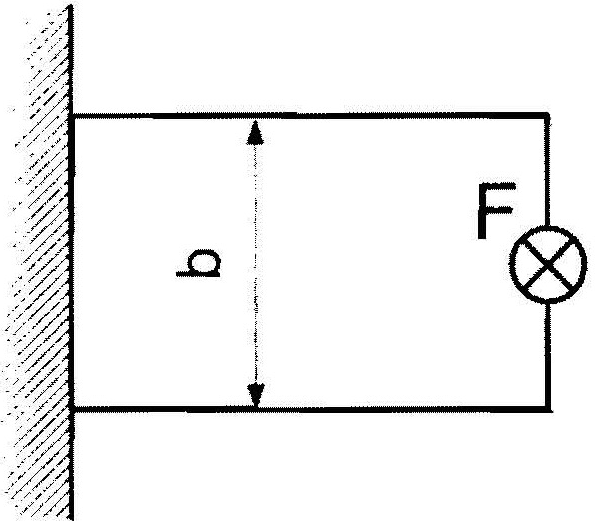
\includegraphics[width=15mm]{federn/blattfedern-rechteck} & const. & $\frac{b\cdot s^2}{6}$ & $\frac{6\cdot F \cdot x}{b\cdot s^2}$ & $\frac{6\cdot F \cdot L}{b \cdot s^2}$ & 4\\
		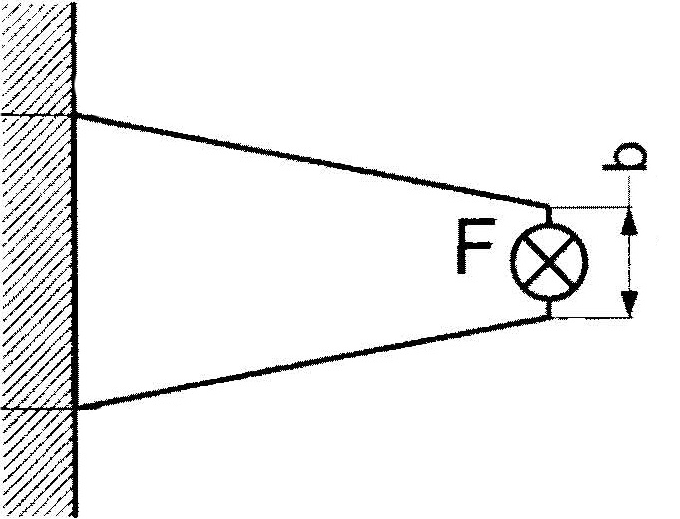
\includegraphics[width=15mm]{federn/blattfedern-trapez} & $b'+\frac{x \cdot (b-b')}{L}$ & $\frac{s^2\cdot [b'+\frac{x}{L}(b-b')]}{6}$ & $\frac{6\cdot F \cdot x}{s^2[b'+\frac{x}{L}(b-b')]}$ & $\frac{6\cdot F \cdot L}{b \cdot s^2}$ & $\frac{12}{2+b'/b}$\\
		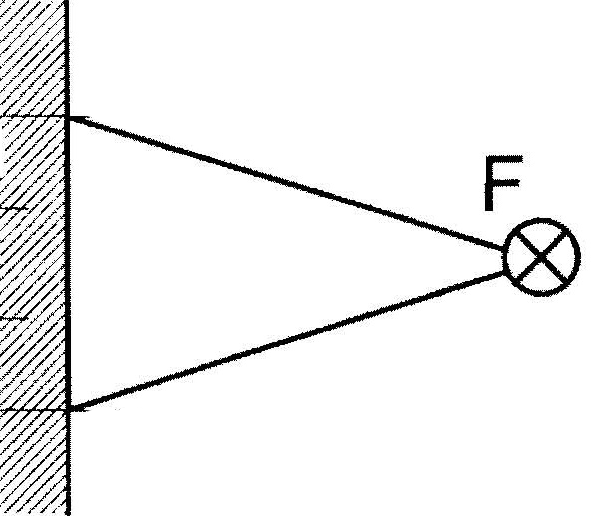
\includegraphics[width=15mm]{federn/blattfedern-dreieck} & $\frac{x \cdot b}{L}$ & $\frac{b\cdot s^2 \cdot x}{6\cdot L}$ & $\frac{6\cdot F \cdot L}{b\cdot s^2}$ & $\frac{6\cdot F \cdot L}{b \cdot s^2}$ & 6\\
    \bottomrule
\end{tabularx}
\\[10pt]
\hrule
% Federrate
\begin{eeqn}{Federrate}
	\begin{align}
		c &= \frac{b\cdot s^3 \cdot E}{q_1 \cdot L^3}
	\end{align}
	Die Federrate ist eine Funktion der Geometrie ($q_1$, $b$ und $s$) und des Werkstoffs $E$.
\end{eeqn}

% Federweg
\begin{eeqn}{Federweg}
	\begin{align}
		f &= q_1 \cdot \frac{L^3}{b\cdot s^3}\cdot \frac{F}{E}
	\end{align}
\end{eeqn}

% max. Federweg
\begin{eeqn}{maximaler Federweg}
	\begin{align}
		f_\text{max} &= q_1 \cdot \sigma_\text{B,zul} \cdot \frac{L^2}{6 \cdot s \cdot E}
	\end{align}
\end{eeqn}

\begin{figure}[H]
	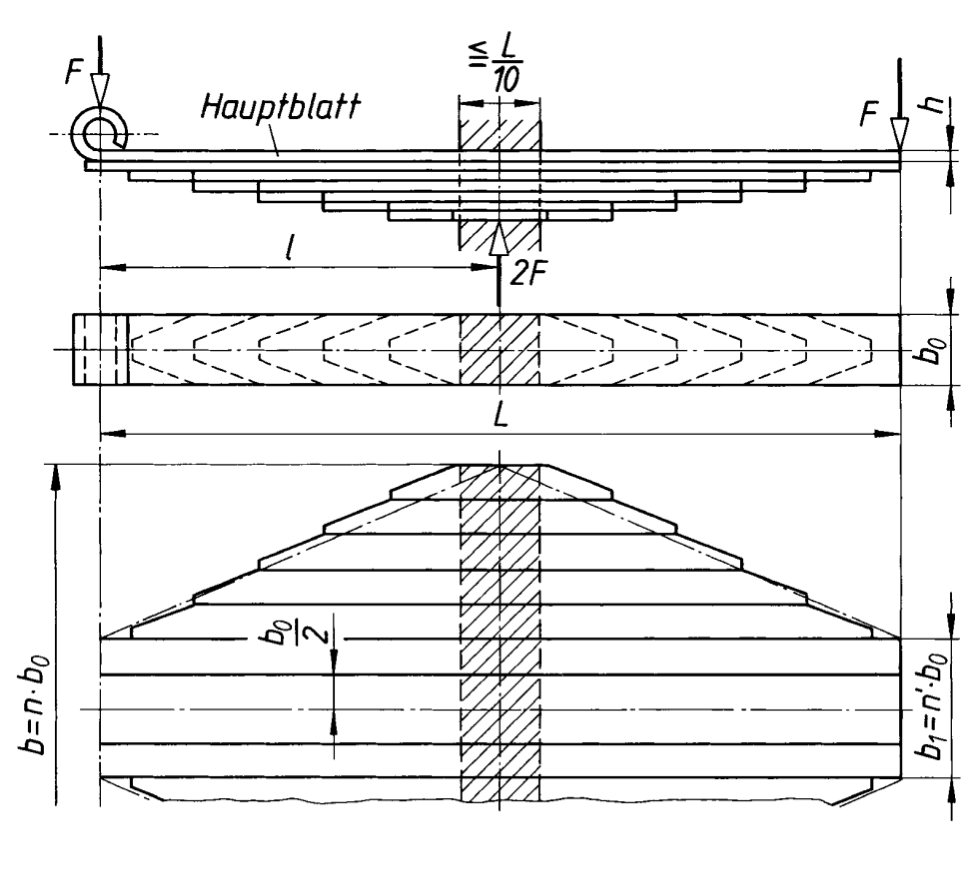
\includegraphics[width=\linewidth]{federn/blattfedern-geschichtet}
	\caption*{Geschichtete Blattfedern}
\end{figure}

% geschichtete Blattfedern
\hrule
\begin{eeqn}{geschichtete Blattfedern}
	Geschichtete Blattfedern verhalten sich wie Trapezfedern mit folgenden Einschränkungen:
	\begin{align}
		&q_1  = \frac{12}{2+\frac{z'}{z}}\\
		&b' = z'\cdot b_0 \\
		&b  = z \cdot b_0
	\end{align}
\end{eeqn}

\subsection{Drehfedern (Biegefedern)}
\begin{vardef}
	\item[$L$] Länge der abgewickelten Feder (Drahtlänge)
	\item[$L^*$] Länge einer Windung
	\item[$i_\text{F}$] Anzahl der Windungen
	\item[$\alpha_0$] Winkel der Federenden zueinander.
	\item[$a$] Abstand der unbelasteten Windungen (in Rad)
	\item[$d$] Drahtdurchmesser
	\item[$D_\text{a}$] Außendurchmesser der Feder
	\item[$D_\text{i}$] Innendurchmesser der Feder
	\item[$D_\text{m}$] Mittlerer  Durchmesser der Feder
	\item[$L_\text{K}$] Gesamtlänge des Federkörpers
\end{vardef}
\begin{figure}[H]
	\centering
	\begin{minipage}[b]{0.45\linewidth}
		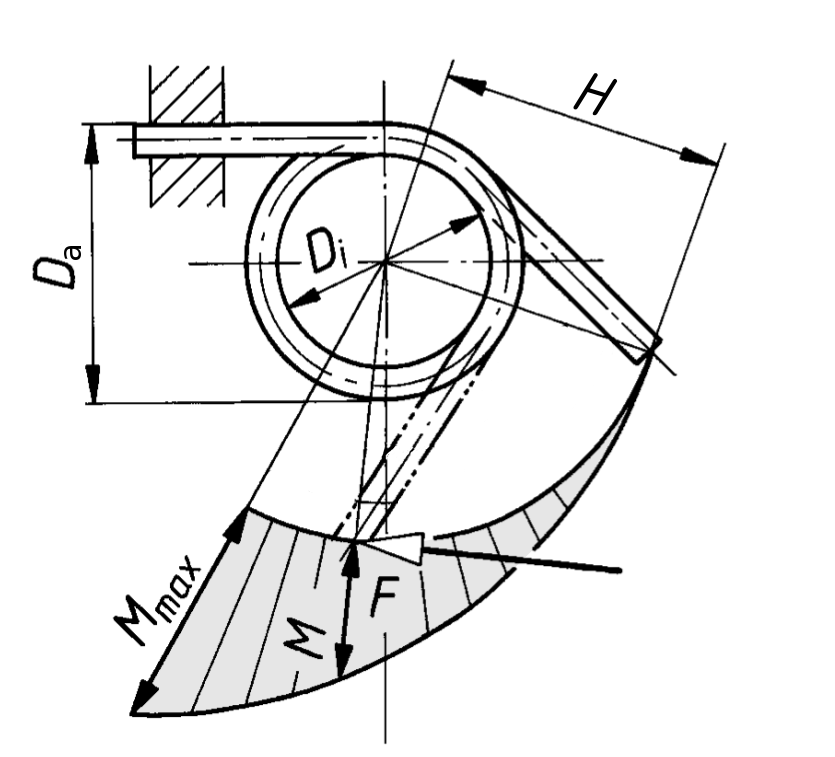
\includegraphics[width=\linewidth]{federn/drehfedern}
		\caption*{Belastung einer Drehfeder}
	\end{minipage}
	\begin{minipage}[b]{0.45\linewidth}
		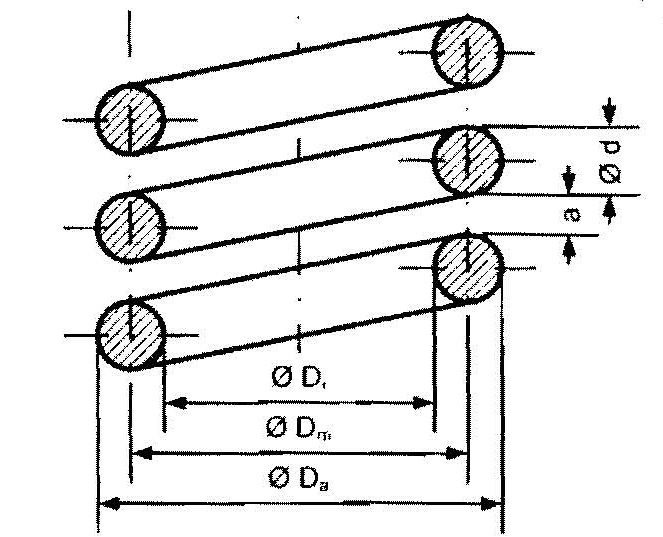
\includegraphics[width=\linewidth]{federn/drehfedern-geometrie}
		\caption*{Geometrie einer Drehfeder}
	\end{minipage}
\end{figure}

\hrule
% Wicklungsverhältnis
\begin{eeqn}{Wicklungsverhältnis}
	\begin{align}
		W &= \frac{D_m}{d}
	\end{align}
\end{eeqn}

% Federgeometrie
\begin{eeqn}{Federgeometrie}
	\label{sec:federgeometrie-drehfedern}
	\begin{align}
		& D_\text{a} = D_\text{m} + d \\
		& D_\text{i} = D_\text{m} - d \\
		& L = i_\text{F} \cdot L^*
	\end{align}
\end{eeqn}

% Länge einer Windung
\begin{eeqn}{Länge einer Windung}
	Wenn $(a+d) \leq 0,25\cdot D_\text{m}$, dann gilt:
	\begin{align}
         L^* &= \pi \cdot D_\text{m}
    \end{align}
    anderenfalls gilt:
    \begin{align}
    	L^* = \sqrt{(D_\text{m}\cdot\pi)^2+(a+d)^2}
    \end{align}
\end{eeqn}

% Korrekturfaktor durch Spannnungserhöhungen an der Innenseite
\begin{eeqn}{Korrekturfaktor durch Spannnungserhöhungen an der Innenseite}
	\begin{align}
		q & = \frac{W+0,07}{W-0,75}
	\end{align}
	Beim Auslegen von Federn wird $q=1$ gesetzt, später wird dann der tatsächliche Wert von $q$ bestimmt.
\end{eeqn}

% Spannungen in der Feder
\begin{eeqn}{Spannungen in der Feder}
	\begin{align}
		\sigma_\text{B} & = \frac{F\cdot H \cdot 32}{\pi \cdot d^3} \cdot q
	\end{align}
	Hierbei entspricht $H$ dem Hebelarm, welcher die Kraft $F$ zum Mittelpunkt der Feder aufweist. Alternativ kann auch $M = F\cdot H$ gesetz werden.
\end{eeqn}

% Federrate
\begin{eeqn}{Federrate}
	\begin{align}
		c & = \frac{I_\text{ax}\cdot E}{L} = \frac{M}{\alpha}
	\end{align}
\end{eeqn}

% Winkel der Federenden
\begin{eeqn}{Winkel der Federenden zueinander}
		Die Nachkommerstellen von $i_\text{F}$ geben an, in welchem Winkel die Enden der Feder zueinander stehen. Diesen Winkel nennt man auch gewickelten Grundwinkel.
		\begin{figure}[H]
			\centering
			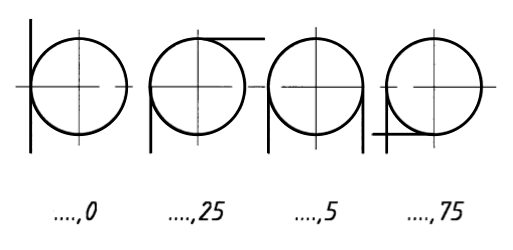
\includegraphics[width=0.75\linewidth]{federn/drehfedern-winkel}
		\end{figure}
\end{eeqn}

% Gesamtlänge Federkörper
\begin{eeqn}{Gesamtlänge Federköper}
	Bei anliegenden Windungen:
	\begin{align}
		L_\text{K} &= (i_\text{F}+1,5)\cdot d
	\end{align}
	Bei Windungsabstand:
	\begin{align}
		L_\text{K} &= i_\text{F} \cdot (a+d) +d
	\end{align}
\end{eeqn}

\pagebreak
\subsection{Drehstabfedern}
\begin{vardef}
	\item[$l_\text{k}$] Kopflänge
	\item[$l_\text{f}$] federnde Länge (Länge eines reinen Torsionsstab, der die selbe Federwirkung hätte)
	\item[$l_\text{h}$] Hohlkehlenlänge
	\item[$l_\text{e}$] Ersatzlänge 	
	\item[$l_\text{k}$] Kopflänge
	\item[$d$] Durchmesser im federnden Bereich
\end{vardef}
\begin{figure}[H]
	\centering
	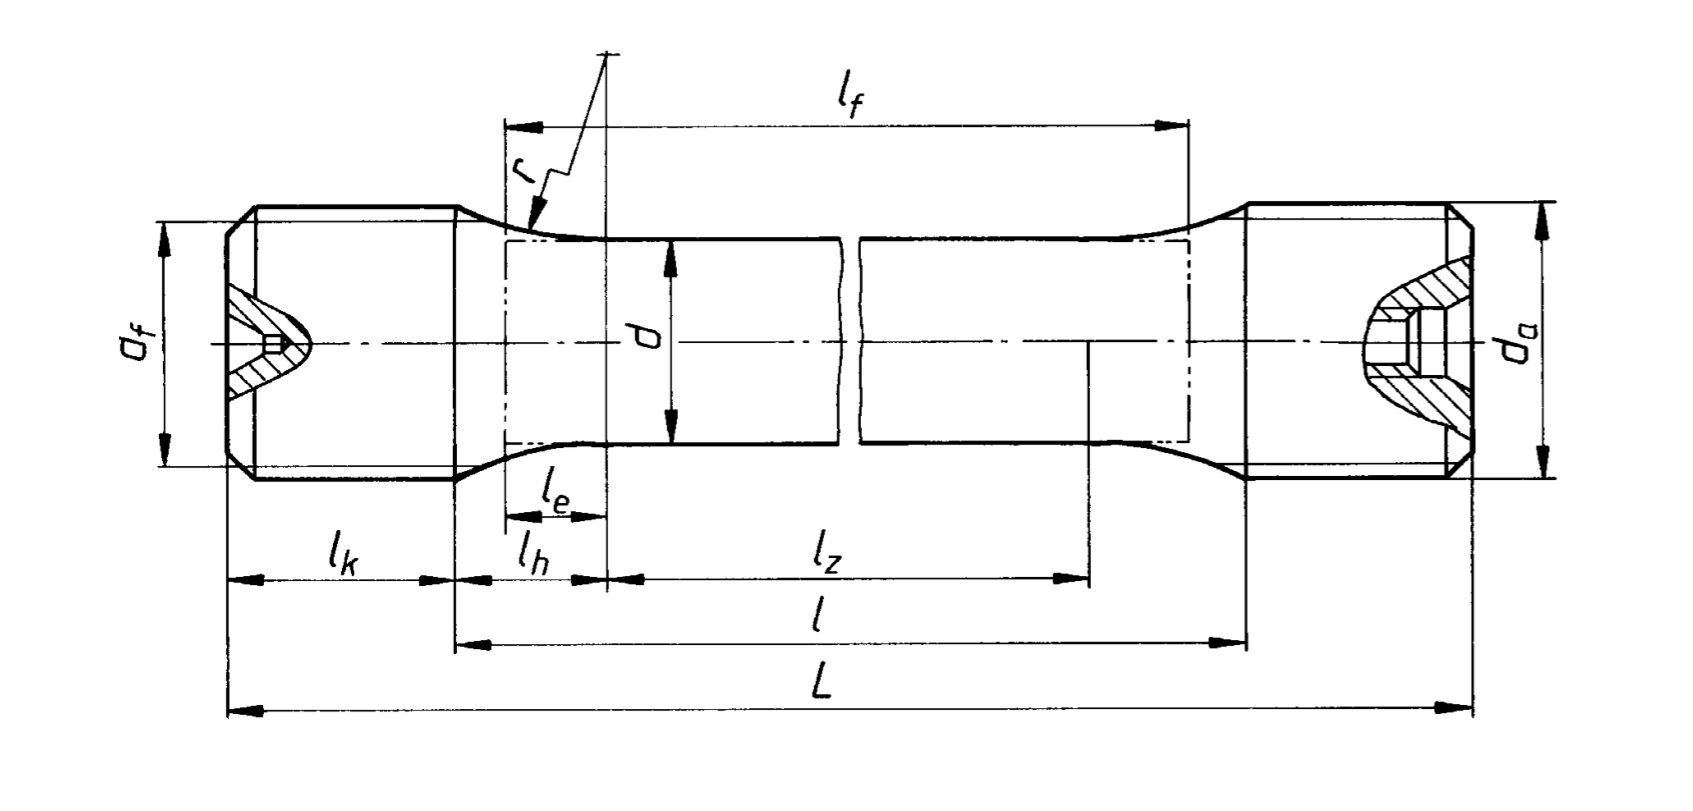
\includegraphics[width=0.8\linewidth]{federn/drehstabfeder}
	\caption*{Drehstabfeder}
\end{figure}

\hrule
% Federgeometrie
\begin{eeqn}{Federgeometrie}
	\begin{align}
		& l_\text{h} = \frac{d_\text{f}-d}{2}\cdot \sqrt{\frac{4r}{d_\text{f}-d}-1} \\
		& l_\text{z} = l- 2\cdot l_\text{h} \\
		& l_\text{e} = \nu \cdot l_\text{h}\\
		& l_\text{f} = l_\text{z} + 2\cdot l_\text{e}
	\end{align}
\end{eeqn}

% Federrate
\begin{eeqn}{Federrate}
	\begin{align}
		c &= \frac{M_\text{t}}{\alpha} = \frac{G\cdot I_\text{p}}{l_\text{f}}
	\end{align}
\end{eeqn}

% Auslegung der Feder
\begin{eeqn}{Auslegung der Feder}
	Die maximale Belastung der Feder ergibt sich aus der maximalen Torsionsspannung, die aus der Verdrillung resultiert.
	\begin{align}
		M_\text{max} &= \tau_\text{zul} \cdot \frac{\pi \cdot d^3}{16}
	\end{align}
\end{eeqn}

\subsection{Schraubenfedern (Zug-/Druckfedern)}
\begin{vardef}
	\item[$s^*$] Federweg pro Windung
	\item[$s$] Federweg der gesamten Feder 
	\item[$d$] Drahtdurchmesser
	\item[$D_\text{m}$] Mittlerer Durchmesser der Feder
	\item[$S_\text{a}$] Restspielsumme (Sicherheitsabstand)
	\item[$i_\text{s}$] Anzahl der eingerollten oder eingeschraubten Windungen
	\item[$L_\text{c}$] Blocklänge der Feder (Alle Windungen liegen aufeinander)
	\item[$L_\text{n}$] Nennlänge der Feder (minimale Federlänge)
	\item[$i_\text{G}$] Gesamtwindungszahl
	\item[$i_\text{F}$] Anzahl federnder Windungen
\end{vardef}

\hrule
% Federgeometrie
\begin{eeqn}{Federgeometrie}
	\vspace{5pt} siehe \ref{sec:federgeometrie-drehfedern} auf Seite \pageref{sec:federgeometrie-drehfedern}
\end{eeqn}

% Federrate
\begin{eeqn}{Federrate}
	\begin{align}
		c &= \frac{G \cdot d^4}{8\cdot i_\text{F} \cdot D_\text{m}^3}
	\end{align}
\end{eeqn}

% Federkraft
\begin{eeqn}{Federkraft}
	\begin{align}
		F &= c \cdot s \qquad \text{$s$ ist der Federweg} 
	\end{align}
\end{eeqn}

% Federweg
\begin{eeqn}{Federweg}
	\begin{align}
		& s^* = \frac{8\cdot F \cdot D_\text{m}^3}{G\cdot d^4} \\
		& s = i_\text{F} \cdot s^*
	\end{align}
\end{eeqn}

% Wicklungsverhältnis
\begin{eeqn}{Wicklungsverhältnis}
	\begin{align}
		W &= \frac{D_m}{d}
	\end{align}
\end{eeqn}

% Korrekturfaktor
\begin{eeqn}{Korrekturfaktor durch Spannnungserhöhungen an der Innenseite}
	\begin{align}
		q & = \frac{W+0,5}{W-0,75}
	\end{align}
	Beim Auslegen von Federn wird $q=1$ gesetzt, später wird dann der tatsächliche Wert von $q$ bestimmt.
\end{eeqn}

\enlargethispage{\baselineskip}

% Spannungen in der Feder
\begin{eeqn}{Spannungen in der Feder}
	Alle Spannungen in der Feder ausschließlich durch Torsion:
	\begin{align}
		\tau_\text{t} &= q \cdot \frac{8 \cdot F \cdot  D_\text{m}}{\pi \cdot d^3}
	\end{align}
	Das in diesem Belastungsfall wirkende Moment ergibt sich aus:
	\begin{align}
		M_\text{t} &= F \cdot \frac{D_\text{m}}{2}
	\end{align}
\end{eeqn}

% Kaltgeformte Druckfedern
\begin{eeqn}{Kaltgeformte Druckfedern}
	\begin{align}
		& i_\text{g} = i_\text{f} +2 \\
		& S_\text{a} = i_\text{f}\cdot \left(0,0015\cdot \frac{D_\text{m}^2}{d}+0,1\cdot d\right)\\
		& L_\text{n} = L_\text{C} + S_\text{a}\\
		\intertext{angelegte Enden:}
		& L_\text{C} = (i_\text{g}+1,5) \cdot d
		\intertext{angelegte und plangeschliffene Enden:}
		& L_\text{C} = i_\text{g} \cdot d
		\intertext{ungespannte Länge der Feder:}
		& L_0 = L_n + \frac{F}{c} \\ 
		\intertext{man braucht $F$ zum erreichen der minimalen Nennlänge}
		\intertext{Blockkraft:}
		& F_c = F + c \cdot S_a \\  
		\intertext{man braucht $F$ zum erreichen der minimalen Nennlänge}
	\end{align}
\end{eeqn}

% Warmgeformten Druckfedern
\begin{eeqn}{Warmgeformte Druckfedern}
	\begin{align}
		& i_\text{g} = i_\text{f} +1,5 \\
		& S_\text{a} = 0,02 \cdot D_\text{a} \cdot i_\text{f} 
		\intertext{angelegte Enden:}
		& L_\text{C} = (i_\text{g}+1,1) \cdot d
		\intertext{angelegte und plangeschliffene Enden:}
		& L_\text{C} = (i_\text{g}-0,3) \cdot d
	\end{align}
\end{eeqn}


% Warmgeformten Zugfedern
\begin{eeqn}{Warmgeformte Zugfedern}
	abgebogene Ösen:
	\begin{align}
		& i_\text{g} = i_\text{f} \\
		& L_\text{C} = (i_\text{g}+1) \cdot d
	\end{align}
	eingerollt oder eingeschraubte Enden:
	\begin{align}
		i_\text{g} = i_\text{f} + i_\text{s}
	\end{align}
	Ösen:
	\begin{align}
		\text{Parallel} &\quad i_\text{f} = x,0~\text{oder}~x,5 \\ 
		\text{Versetzt} &\quad i_\text{f} = x,25~\text{oder}~x,75	\end{align}
\end{eeqn}
